\chapter{Diseño e Implementación del sistema basado en IoT}\label{cap: }

\addcontentsline{toc}{section}{Introducción}
        \textbf{\Large Introducción}\newline
        
    En este capítulo se comentan los pasos seguidos para la implementación del sistema: se realiza la descripción del proceso a monitorear o planta, los sensores que incorpora...

\section{Descripción del sistema} \label{descripcion_sistema}

    El sistema de supervisión se implementa sobre una prueba de concepto desarrollada para llevar a cabo la toma de la data de los sensores incorporados durante 4 meses para facilitar el continuar con la investigación e inferir los daños que las diferentes variables (temperatura, humedad, ruido y CO2) inciden en el deterioro de los objetos de la colección para los diferentes materiales que en ella se encuentran; esto según el análisis teórico desarrollado a lo largo del capítulo primero.

    Esta prueba de concepto (figura \ref{imag:prueba_concepto}) se dividió en 3 submódulos. En el submódulo 1 se encuentra el microcontrolador principal, en este caso un NodeMCU que tendrá interconectado a su vez un shield DS3231, un reloj de tiempo real para almacenar la fecha y hora de cada medición que se realice, así como un sensor SGP30 para la captura de los valores de CO2 dentro de la vitrina; estos datos son almacenados en una tarjeta SD por un shield de lector para este tipo de almacenamiento, además de contar con un sistema de respaldo interno de 2 baterías de litio para su funcionamiento continuo aunque existan fallos eléctricos, además de que las ubicaciones de las vitrinas se encuentre alejada de una toma de corriente eléctrica.

    Sin embargo, para casos extremos energéticos se agregó el submódulo 2 el cual es una batería de tipo power bank de 10A que va conectado también al submódulo 1 y puede ser recargado simultáneamente.

    Por su parte en el submódulo 3 se encuentran los 2 sensores para medir la temperatura, la humedad (DHT22) y el ruido a través de un sensor Grove de micrófono.\\
    
    \begin{figure}[H]
      \centering
      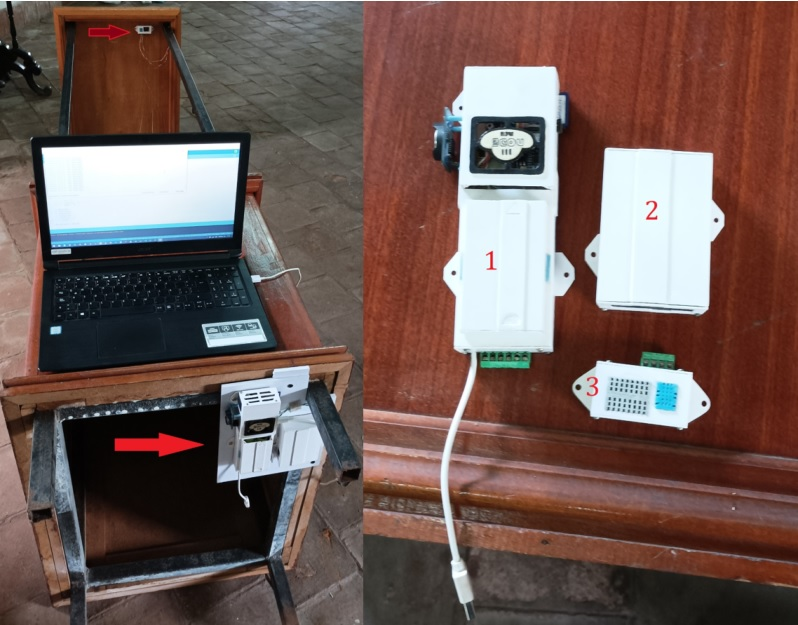
\includegraphics[width=7.5cm, height=6cm]{imagenes/prueba_concepto.jpg}
      \caption{Prueba de Concepto}
      \label{imag:prueba_concepto}
    \end{figure}

    Los submódulos fueron instalados en una sola vitrina y de manera separada a conveniencia de los investigadores y los especialistas del museo, el submodulo 1 y 2 se optó por ubicarlos en la parte baja de la vitrina (figura \ref{imag:ubicacion_submodulos1y2_vitrina}) en aras de que no rompiera el ambiente artístico de la colección,
    y el submódulo 3 es ubicado en la parte superior de la vitrina (figura \ref{imag:ubicacion_submodulo3}) para recolectar la mayor cantidad de información posible.

    \begin{figure}[H]
        \centering
        \begin{subfigure}[b]{0.45\linewidth}
        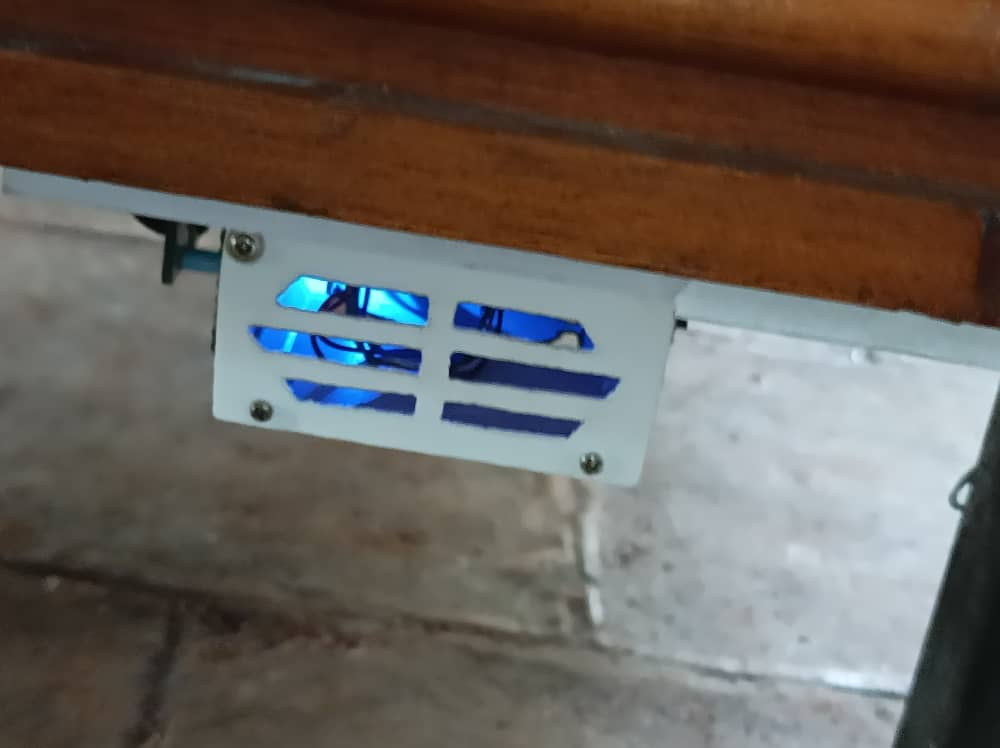
\includegraphics[width=\linewidth]{imagenes/submodulo 1.jpg}
        \caption{Ubicación submódulo 1}
        \label{imag:ubicacion_submodulo1}
    \end{subfigure}
    \begin{subfigure}[b]{0.45\linewidth}
        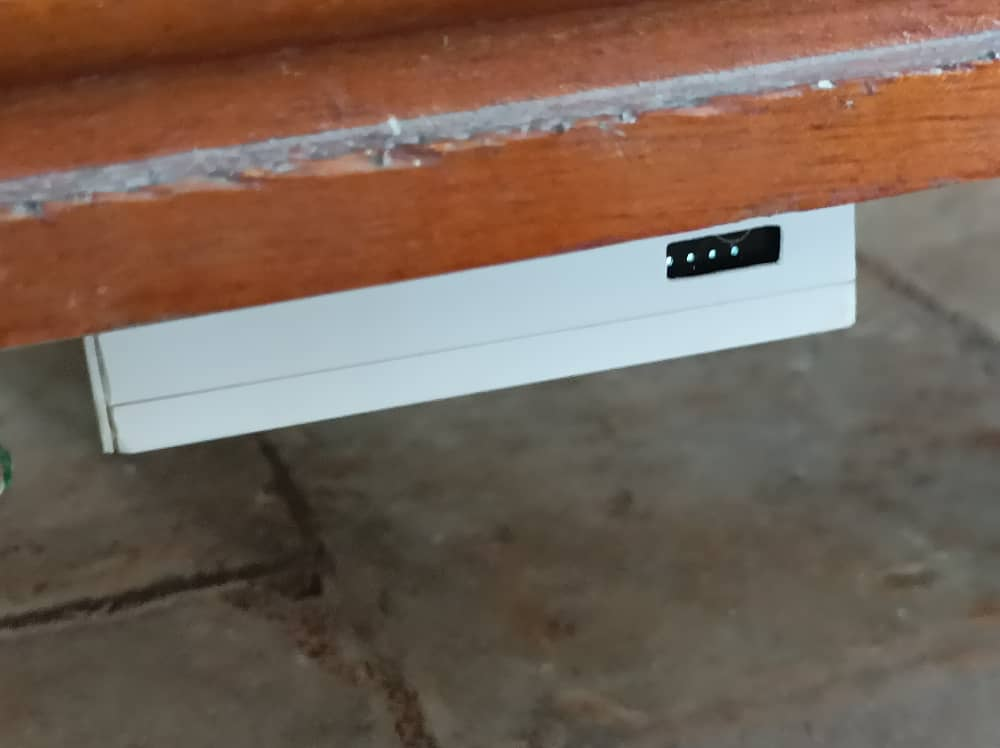
\includegraphics[width=\linewidth]{imagenes/submodulo 2.jpg}
        \caption{Ubicación submódulo 2}
        \label{imag:ubicacion_submodulo2}
    \end{subfigure}
        \caption{Ubicación de los submódulos 1 y 2 en la vitrina}
        \label{imag:ubicacion_submodulos1y2_vitrina}
    \end{figure}

    \begin{figure}[H]
        \centering
        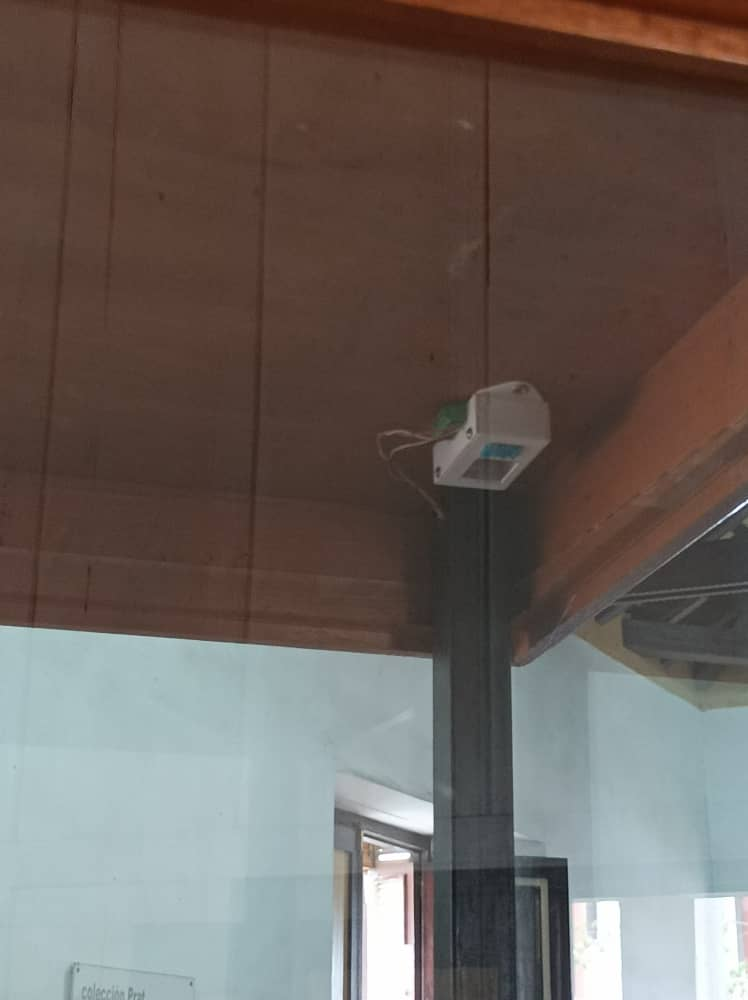
\includegraphics[width=7cm, height=6cm]{imagenes/submodulo 3.jpg}
        \caption{Ubicación submódulo 3}
        \label{imag:ubicacion_submodulo3}
      \end{figure}

\section{Sensores} \label{sec:sensores}

    La secuencia de sensores pertenecientes al sistema es selecta, puesto que se tomaron los sensores teniendo en cuenta varios elementos:

    \begin{itemize}
        \item Variable a medir
        \item Rango de medición
        \item Precisión
        \item Voltaje de alimentación
        \item Corriente de alimentación
        \item Precio
    \end{itemize}

En la tabla \ref{tab:relacion_sensores} se relaciona el sensor a emplear según la variable a medir.

    \begin{table}[h]
        \centering
        \caption{Relación sensores}
        \label{tab:relacion_sensores}
        \begin{tabular}{|l|l|l|}
        \hline
        \cellcolor[HTML]{9698ED}                      & \cellcolor[HTML]{9698ED}                           & \cellcolor[HTML]{9698ED}                         \\
        \multirow{-2}{*}{\cellcolor[HTML]{9698ED}No.} & \multirow{-2}{*}{\cellcolor[HTML]{9698ED}Variable} & \multirow{-2}{*}{\cellcolor[HTML]{9698ED}Sensor} \\ \hline
        1                                             & Temperatura                                        & DHT22                                            \\ \hline
        2                                             & Humedad                                            & DHT22                                            \\ \hline
        3                                             & CO2                                                & SGP30                                            \\ \hline
        4                                             & Vibración                                          & TZT-LM393                                        \\ \hline
        5                                             & Calidad de Aire                                    & ZP07-MP503                                       \\ \hline
        6                                             & Intensidad luminosa                                & BH1750                                           \\ \hline
        \end{tabular}
    \end{table}

Estos sensores estarán dispuestos en zonas específicas dentro de la colección, dígase en vitrinas o, para la captura de datos, en las salas.
Esto permite tener datos de dentro de las vitrinas y compararlos con los datos recolectados de las salas en general, posibilitando el análisis de las diferencias entre los máximos y mínimos de los valores recolectados.
    
A continuación se analizan las características técnicas de cada sensor teniendo en cuenta los elementos descritos anteriormente.

\subsection{Sensor de temperatura y humedad DHT22}\label{sub:dht22}

    \begin{figure}[H]
      \centering
      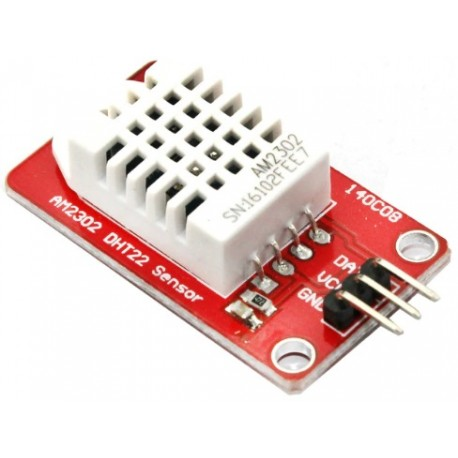
\includegraphics[width=5cm, height=5cm]{imagenes/dht22.jpg}
      \caption{Sensor DHT22}
      \subcaption*{Fuente: Datasheet fabricante}
      \label{imag:dht22}
    \end{figure}

Este sensor se encuentra presente en el submódulo 3 (ver figura \ref{imag:prueba_concepto}) ubicado en la parte superior de la vitrina,
logrando así obtener la mayor cantidad de valores de temperatura y humedad.
   
El DHT22 (AM2302) es un sensor digital de temperatura y humedad relativa de buen rendimiento y de bajo costo. Integra un sensor capacitivo de humedad y un termistor para medir el aire circundante, y muestra los datos mediante una señal digital en el pin de datos (no posee salida analógica).

Utiliza tecnología exclusiva de recolección de señales digitales y tecnología de detección de humedad, lo que garantiza su confiabilidad y estabilidad. Sus elementos de detección están conectados con una computadora de un solo chip de 8 bits.\\

\textbf{Especificaciones ténicas}

\begin{itemize}
    \item Modelo: AM2302
    \item Voltaje de alimentación: 3.3-6V DC
    \item Señal de salida: señal digital
    \item Rango: humedad de 0 - 100\%HR || temperatura de -40 - 125°C
\end{itemize}

\begin{figure}[H]
    \centering
    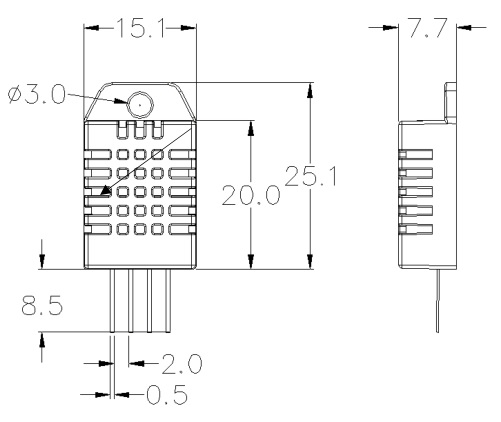
\includegraphics[width=8cm, height=6cm]{imagenes/dht22 dimensiones.jpg}
    \caption{Dimensiones sensor DHT22}
    \subcaption*{Fuente: Datasheet fabricante}
    \label{imag:dimensiones_dht22}
\end{figure}

Secuencia de números de pines: De izquierda a derecha 1,2,3,4 (tabla \ref{tab:pines_DHT})

\begin{table}[H]
    \centering
    \caption{Distribución pines DHT22}
    \label{tab:pines_DHT}
    \begin{tabular}{|l|l|}
    \hline
    Pin & Función            \\ \hline
    1   & VDD - Alimentación \\ \hline
    2   & DATA - Señal       \\ \hline
    3   & NULL               \\ \hline
    4   & GND                \\ \hline
    \end{tabular}
\end{table}

\subsection{Sensor de CO2 SGP30}

\begin{figure}[H]
      \centering
      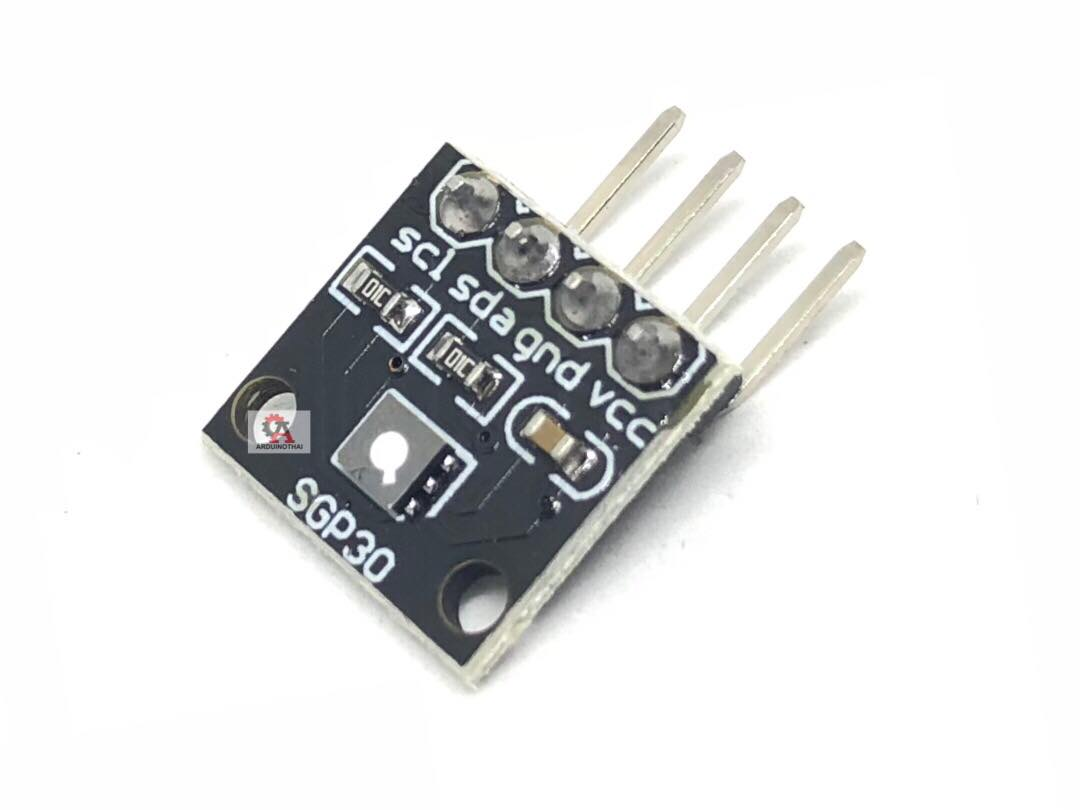
\includegraphics[width=6cm, height=4.5cm]{imagenes/sgp30.jpg}
      \caption{Sensor SGP30}
      \label{imag:sgp30}
\end{figure}

Este sensor se encuentra ubicado en el submódulo 3 (figura \ref{imag:prueba_concepto}) en la parte superior de la vitrina, esto debido a que los gases tienden a subir \textbf{(referenciar)} y de esta manera se obtienen los valores de CO2 más exactos.

...

\subsection{Sensor de vibración TZT-LM393}

\textbf{Imagen}

\newpage

\subsection{Sensor de calidad de aire ZP07-MP503}

\vspace{1cm}

\begin{figure}[H]
      \centering
      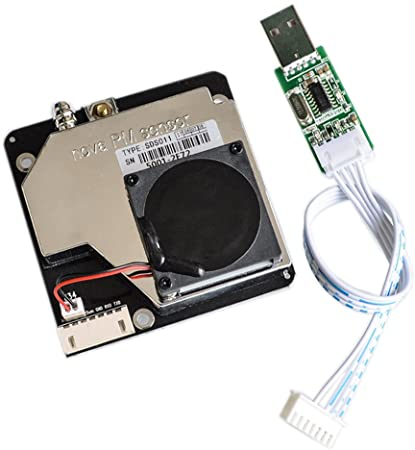
\includegraphics[width=4.5cm, height=4.5cm]{imagenes/Sensor SDS011.jpg}
      \caption{Sensor SDS011}
      \label{imag:SDS011}
   \end{figure}

Se basa en el principio de dispersión láser: se puede inducir la dispersión de la luz cuando las partículas atraviesan el área de detección. La luz dispersa se transforma en señales eléctricas, después estas señales serán amplificadas y procesadas. El número y el diámetro de las partículas se pueden obtener mediante análisis porque la forma de onda tiene ciertas relaciones con el diámetro de las partículas.\\

\textbf{Otros datos}

\begin{itemize}
    \item Corriente del sueño: 2mA
    \item Frecuencia de muestreo serie: 1 segundo
    \item Resolución diámetro de partículas: <= 0.3um
    \item Rango de temperatura: -20 a 50°C
    \item Tamaño físico: 71mm x 70mm x 23mm 
\end{itemize}

\vspace{5cm}

\subsection{Sensor de luz BH1750}

El Módulo BH1750 es un sensor de iluminación digital para medición de flujo luminoso (iluminancia) de la empresa Rohm Semiconductor. Componente que posee dentro de su arquitectura interna, un conversor análogo digital (ADC) de 16 bits con una salida digital de formato I2C, que facilita la integración con microcontroladores o sistemas embebidos diversos. Este módulo entrega la intensidad luminosa directamente en unidades de Lux que es equivalente a Lumen/m2.\\

\begin{figure}[H]
    \centering
    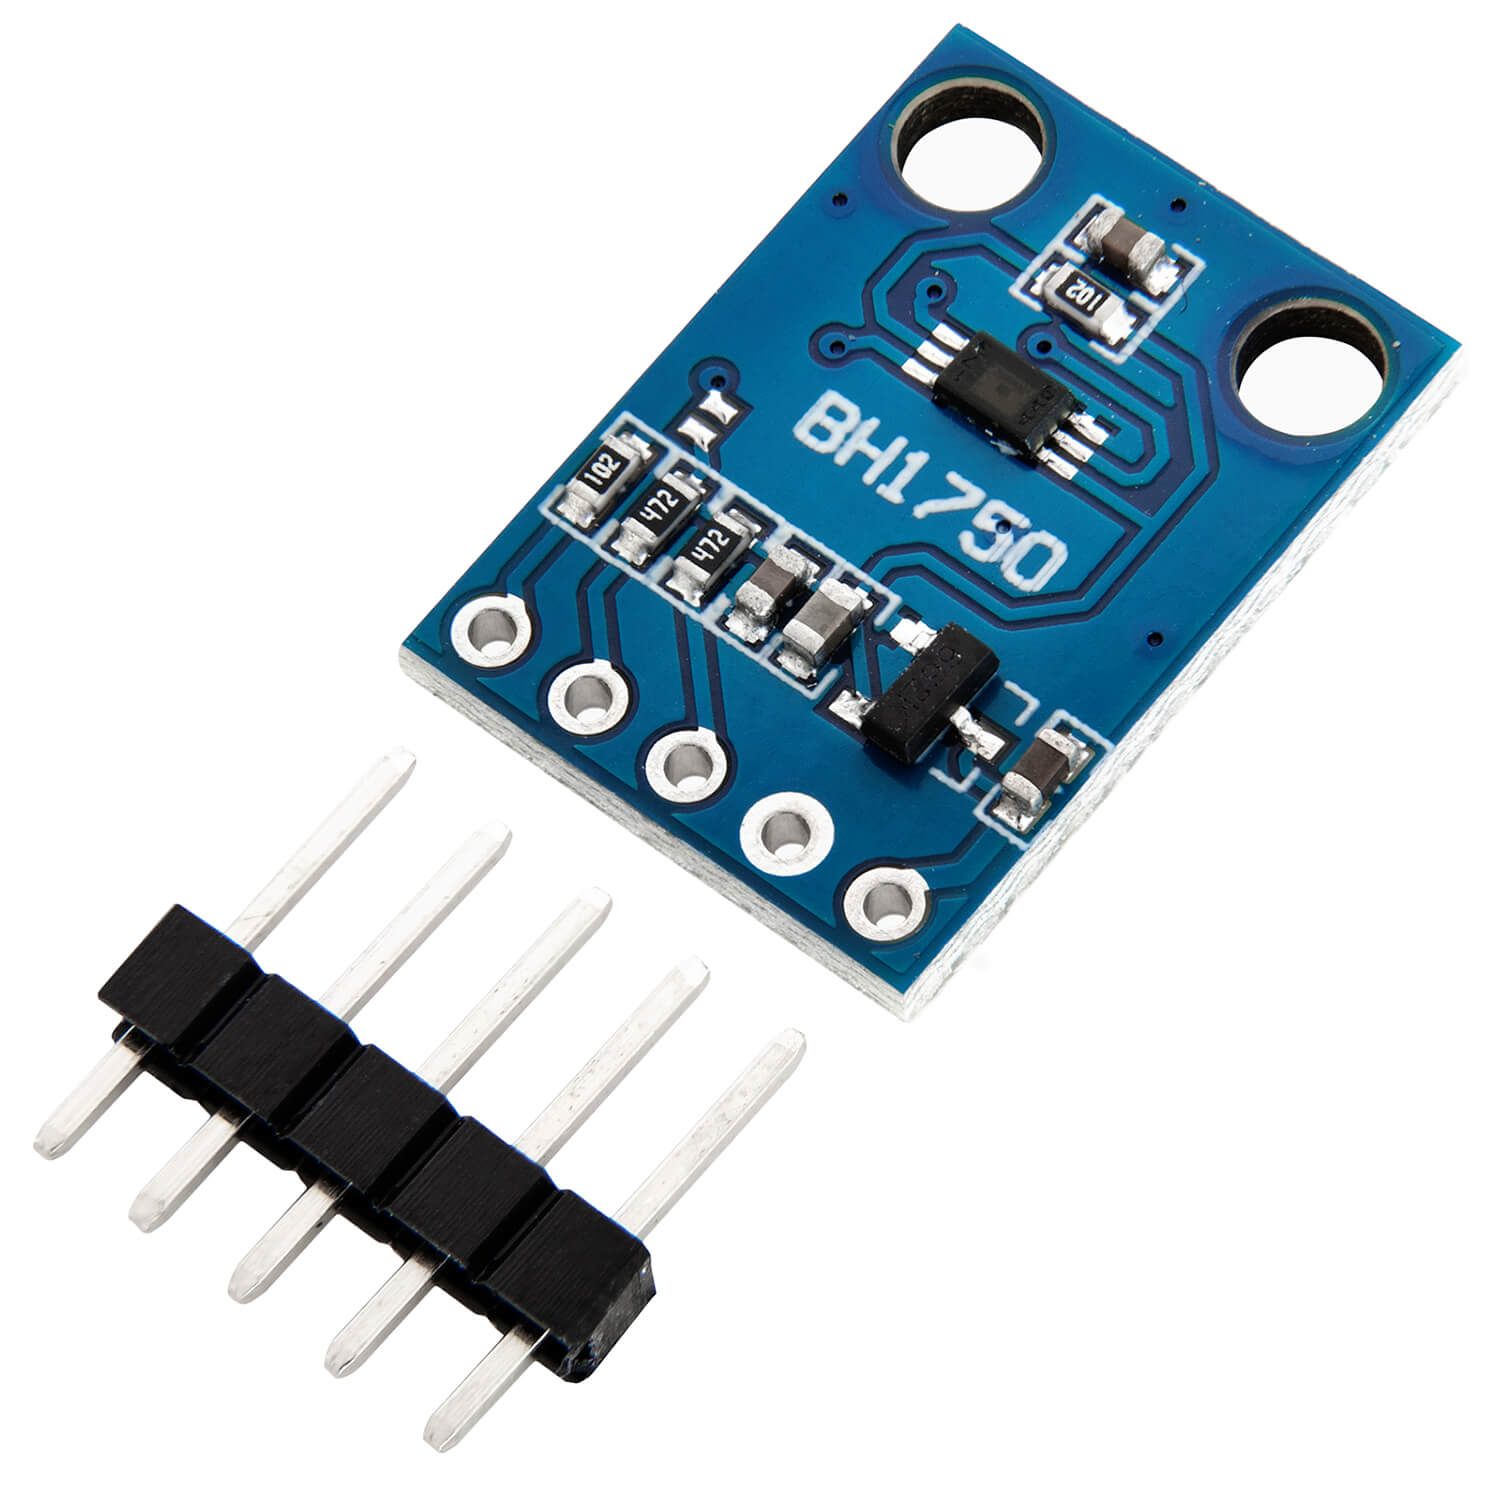
\includegraphics[width=5cm, height=4cm]{imagenes/Sensor BH1750.jpg}
    \caption{Sensor BH1750}
    \label{imag:BH1750}
 \end{figure}

\textbf{Otros datos}

\begin{itemize}
    \item Interfaz Digital: I2C
    \item Frecuencia máxima de transmisión: 400kHZ
    \item Temperatura de operación: Desde -40°C hasta 85°C
\end{itemize}

Para su correcto funcionamiento, este sensor debe ir acompañado de una serie de componentes electrónicos para su acondicionamiento.
En la figura \ref{imag:acondicionamiento_BH1750} se puede observar el acondicionamiento brindado por el fabricante.

\begin{figure}[H]
    \centering
    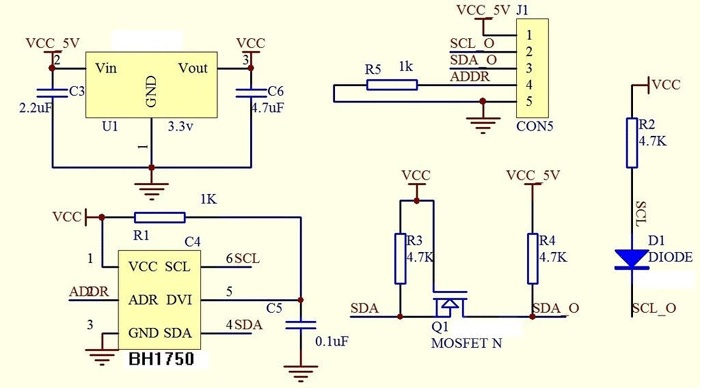
\includegraphics[width=11cm, height=7cm]{imagenes/acondicionamientos sensor BH1750.jpg}
    \caption{Acondicionamiento sensor BH1750}
    \subcaption*{Fuente: Datasheet fabricante}
    \label{imag:acondicionamiento_BH1750}
\end{figure}

\vspace{1cm}

\subsection{Alimentación}

\textbf{Regulador LDO RT9013.}\newline

El RT9013 es un regulador LDO de 500 mA de alto rendimiento que ofrece PSRR extremadamente alto y caída ultrabaja. Ideal para aplicaciones inalámbricas y de RF portátiles con requisitos exigentes de rendimiento y espacio.\\

La corriente de reposo RT9013 es tan baja como 25uA, lo que prolonga aún más la vida útil de la batería. El RT9013 también funciona con condensadores cerámicos de baja ESR, lo que reduce la cantidad de espacio de placa necesario para las aplicaciones de energía, lo que es fundamental en los dispositivos inalámbricos de mano.\\

El RT9013 consume 0.7uA típicos en modo de apagado y tiene un tiempo de encendido rápido de menos de 40us. Las otras características incluyen voltaje de caída ultrabajo, alta precisión de salida, protección de limitación de corriente y alta relación de rechazo de ondulación. Disponible en el paquete SC-82, SOT-23-5, SC-70-5 y WDFN-6L 2x2.\\

\textbf{Características}

\begin{itemize}
    \item Amplios rangos de voltaje de operación: 2.2V a 5.5V
    \item Caída baja: 250mV a 500mA
    \item Ruido ultrabajo para aplicaciones de RF
    \item Respuesta ultrarrápida en transitorios de línea/carga
    \item Protección de limitación de corriente
    \item Protección de apagado térmico
    \item Tasa de rechazo de fuente de alimentación alta
    \item A la salida solo se requiere 1 uF de condensador para la estabilidad
    \item Entrada de apagado controlado por lógica TTL
\end{itemize}

\vspace{1cm}

\begin{figure}[H]
    \centering
    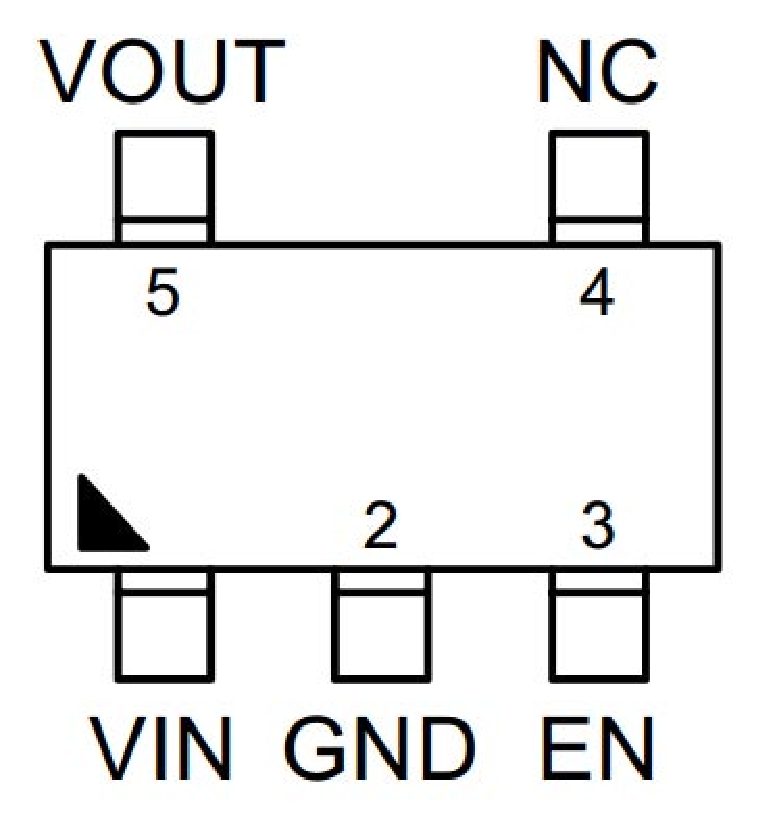
\includegraphics[width=5.5cm, height=6cm]{imagenes/esquematico RT9013.pdf}
    \caption{Configuración de pines}
    \subcaption*{Fuente: Datasheet fabricante}
    \label{imag:pines_RT9013}
\end{figure}

\begin{figure}[H]
    \centering
    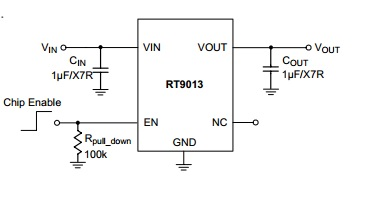
\includegraphics[width=12cm, height=7cm]{imagenes/acondicionamiento RT9013.jpg}
    \caption{Acondicionamiento}
    \subcaption*{Fuente: Datasheet fabricante}
    \label{imag:acondicionamiento_RT9013}
\end{figure}

\newpage

\section{Condiciones medioambientales...} \label{sec: condiciones_medioambientales}


    \begin{figure}[H]
        \centering
        \includegraphics[width=16cm, height=5cm]{imagenes/gráfica_comparativa_variables_medioambientales.png}
        \caption{Correlación de valores medioambientales}
        \subcaption*{Fuente: Elaboración propia}
        \label{imag:grafica_condiciones_medioambientales}
    \end{figure}


\addcontentsline{toc}{section}{Conclusiones}
        \textbf{\Large Conclusiones}\newline
